\section{Evaluation}
\label{sec:eval}

We aimed to measure and evaluate \slog{}'s
improved indexing and data parallelism, using
three sets of performance benchmarks (PBs):

\begin{description}
\item[\textbf{PB1}] (Section~\ref{sec:eval:pb1}) How does \slog{} compare against other systems
  designed for performance and parallelism on traditional Datalog
  workloads (without ADTs): Souffl\'e and RadLog?
\item[\textbf{PB2}] (Section~\ref{sec:eval:pb2}) How do \slog{} subfacts perform against Souffl\'e ADTs
  in the context of the $m$-CFA and $k$-CFA benchmarks developed in Section~4.
\item[\textbf{PB3}] (Section~\ref{sec:eval:pb3}) How well can \slog{} scale to many threads on a supercomputer?
\end{description}

We evaluated \textbf{PB1} and \textbf{PB2} by running a set of
experiments on large cloud machines from Amazon AWS and Microsoft
Azure. For \textbf{PB1}, we ran a set of strong scaling experiments of
transitive closure on large graphs, picking transitive closure as an
exemplary problem to measure end-to-end throughput of deductive
inference at scale. For \textbf{PB2}, we measure the performance of
the implementation of our $k$ and $m$-CFA analyses from
Section~\ref{sec:apps} compared to an equivalent implementation in
Souffl\'e using abstract datatypes (ADTs). We answer \textbf{PB3} by
running experiments on the Theta supercomputer at Argonne National
Supercomputing Lab, scaling a control-flow analysis for the
$\lambda$-calculus to $1000$ threads on Argonne's Theta.

\subsection{Transitive Closure}
\label{sec:eval:tc}
\label{sec:eval:pb1}

We sought to compare \slog{}'s full-system throughput on vanilla
Datalog against two comparable production systems: Souffl\'e and
Radlog. Souffl\'e is engineered to achieve the best-known performance
on unified-memory architectures, and supports parallelism via
OpenMP. Radlog is a Hadoop-based successor to the BigDatalog deductive
inference system, which uses Apache Spark to perform distributed joins
at scale~\cite{rasql}. We originally sought to compare \slog{}
directly against BigDatalog, but found it does not support recent
versions of either Spark or Java (being built to target Java
1.5). Under direction of BigDatalog's authors, we instead used Radlog,
which is currently under active development and runs on current
versions of Apache Spark.

We performed comparisons on an \textsf{Standard\_M128s} instance
rented from Microsoft Azure~\cite{mseries}. The node used in our
experiments has 64 physical cores (128 threads) running Intel Xeon
processors with a base clock speed of 2.7GHz and 2,048GB of RAM. To
directly compare \slog{}, Souffl\'e, and Radlog, we ran each on the
same machine using 15, 30, 60, and 120 threads. We ran \slog{} using
OpenMPI version 4.1.1 and controlled core counts via
\texttt{mpirun}. We compiled Souffl\'e from its Git repository, using
Souffl\'e's compiled mode to compile each benchmark separately to use
the requisite number of threads before execution. Radlog runs natively
on Apache Spark, which subsequently runs on Hadoop. To achieve a fair
comparison against Souffl\'e and \slog{}, we ran Radlog using Apache
Spark configured in local mode; Spark's local mode circumvents the
network stack and runs the application directly in the JVM. We used
three large graphs shown the first column of Table~\ref{tab:single-results}:
\textsc{fb-media} is media-related pages on Facebook,
\textsc{ring10000} is ring graph of 10,000 nodes, and
\textsc{suitesparse} is from the UF Sparse Matrix
Collection~\cite{Davis:2011:UFS:2049662.2049663}. We configured Radlog
according the directions on its website, experimenting with a variety
of partitions (used for shuffling data between phases) to achieve the
best performance we could. Ultimately, we used three times as many
partitions as available threads, except for \textsc{ring10000}, for
which we found higher partition counts caused significantly lower
performance.

\begin{table}
\centering
\caption{Single-node TC Experiments}
\begin{tabular}{m{1.7cm}m{1cm}m{2cm}|cm{.5cm}m{.5cm}m{.5cm}m{.5cm}}
\toprule
\multicolumn{3}{c}{Graph Properties}&& \multicolumn{4}{c}{Time (s) at Process Count} \\
Name & Edges & {\quad$\mid$TC$\mid$} & System & 15 & 30 & 60 & 120 \\
\midrule
\multirow{3}{*}{\textsc{fb-media}} & \multirow{3}{*}{206k} & \multirow{3}{*}{96,652,228} & \slog & 62 & 40 & 21 & \textbf{18} \\
 &&& Souffl\'e & 35 & 33 & 34 & 37 \\
 &&& Radlog & 254 & 295 & 340 & 164 \\
\midrule \midrule
\multirow{3}{*}{\textsc{ring10000}} & \multirow{3}{*}{10k} & \multirow{3}{*}{100,020,001} & \slog & 363 & 218 & 177 & \textbf{115} \\
 &&& Souffl\'e & 149 & 143 & 140 & 141 \\
 &&& Radlog & 464 & 646 & 852 & 1292 \\
\midrule \midrule
\multirow{3}{*}{\textsc{suitesparse}} & \multirow{3}{*}{412k} & \multirow{3}{*}{3,354,219,810} & \slog & -- & 1,593 & 908 & \textbf{671} \\
 &&& Souffl\'e & 1,417 & 1,349 & 1,306 & 1,282 \\
 &&& Radlog & -- & -- & -- & -- \\
\bottomrule
\end{tabular}
\label{tab:single-results}
\end{table}

Table~\ref{tab:single-results} details the results of our single-node
performance comparisons in seconds for each thread count, where each
datapoint represents the best of three runs (lower is
better). Experiments were cut off after 30 minutes. In every case, we
found that \slog{} produced the best performance overall at 120
threads, even compared to Souffl\'e's best time. However, as expected,
our results indicate that Souffl\'e outperforms \slog{} at lower core
counts (below 60). Souffl\'e implements joins with tight loops in
\CC{}, and (coupled with its superior single-node datastructures) this
allows Souffl\'e to achieve better performance than either \slog{} or
Radlog at lower core counts. We found that Radlog did not scale nearly
as well as either Souffl\'e or \slog{}. We expected this would be the
case: both \slog{} and Souffl\'e compile to \CC{}. By comparison,
Radlog's Spark-based architecture incurs significant sequential
overhead due to the fact that it is implemented on top of the JVM and
pays a per-iteration penalty by using Hadoop's aggregation and
shuffling phase. \slog{} also incurs sequential overhead compared to
Souffl\'e due to its distributing results after every iteration,
though results indicate that our MPI-based implementation helps
ameliorate this compared to Radlog.





\subsection{AAMs and CFAs}
\label{sec:eval:aam}
\label{sec:eval:pb2}

 \begin{table*}
 \centering
\caption{Control-Flow Analysis Experimental Results: Slog vs. Souffl\'e}\label{tab:results-aam}
 \begin{tabular}{ccccccccc}
   \toprule 
 & \multirow{2}{*}{Term Sz.}&\multirow{2}{*}{Iters}& \multirow{2}{*}{Cf. Pts}& \multirow{2}{*}{Sto. Sz.}& \multicolumn{2}{c}{$8$ Processes} & \multicolumn{2}{c}{$64$ Processes} \\
 & & & & & \multicolumn{1}{c|}{Slog} & \multicolumn{1}{c||}{Souffl\'e}& \multicolumn{1}{c|}{Slog}& \multicolumn{1}{c}{Souffl\'e}\\
 \midrule 
 \parbox[t]{2mm}{\multirow{6}{*}{\rotatebox[origin=c]{90}{3-$k$-CFA}}}
 & 8 & 1,193 & 98,114 & 23,413 & 00:01 & 01:07 & 0:02 & 00:15\\
 & 9 & 1,312 & 371,010 & 79,861 & 00:02 & 14:47 & 0:03 & 02:56 \\
 & 10 & 1,431 & 1,441,090 & 291,317 & 00:06 & \timeout{} & 0:05 & 45:49 \\
 & 11 & 1,550 & 5,678,402 &  1,107,957 & 00:27 & \timeout{} & 0:16 & \timeout{} \\
 & 12 & 1,669 & 22,541,634 & 4,315,125 & 02:14 & \timeout{} & 1:07 & \timeout{} \\
 & 13 & 1,788 & 89,822,530 & 17,022,965 & 12:17 & \timeout{} & 5:08 & \timeout{} \\
\midrule 
 \parbox[t]{2mm}{\multirow{6}{*}{\rotatebox[origin=c]{90}{4-$k$-CFA}}}
 & 9 & 1,363 & 311,790 & 65,397 & 00:01 & 14:38 & 00:03 & 02:08 \\
 & 10 & 1,482 & 1,197,038 & 229,621 & 00:05 & \timeout{} & 00:05 & 40:30 \\
 & 11 & 1,601 & 4,687,854 & 853,493 & 00:20 & \timeout{} & 00:13 & \timeout{} \\
 & 12 & 1,720 & 18,550,766 & 3,281,909 & 01:40 & \timeout{} & 00:53 & \timeout{} \\
 & 13 & 1,839 & 73,801,710 & 12,859,381 & 08:44 & \timeout{} & 03:58 & \timeout{} \\
 & 14 & 1,958 & 294,404,078 & 50,892,789 & 60:53 & \timeout{} & 35:46 & \timeout{} \\

\midrule 
 \parbox[t]{2mm}{\multirow{6}{*}{\rotatebox[origin=c]{90}{5-$k$-CFA}}}
 & 9 & 1,429 & 203,674 & 50,677 & 00:02 & 05:30 & 0:03 & 001:15 \\
 & 10 & 1,548 & 756,890 & 167,285 & 00:04 & 65:20 & 0:04 & 015:08 \\
 & 11 & 1,667 & 2,911,898  & 597,493 & 00:13 & \timeout{} &  0:08 & 196:06 \\
 & 12 & 1,786 & 11,416,218 & 2,245,109 & 00:56 &  \timeout{}& 0:27 & \timeout{} \\
 & 13 & 1,905 & 45,202,074 & 8,687,605 & 04:38 &  \timeout{}& 2:00 & \timeout{} \\
 & 14 & 2,024 & 179,882,650 & 34,158,581 & 25:14 & \timeout{}& 9:58 & \timeout{}\\
\midrule 
 \parbox[t]{2mm}{\multirow{6}{*}{\rotatebox[origin=c]{90}{10-$m$-CFA}}}
 & 50 & 6,120 & 21,005 & 656,847 & 00:02  & 00:02 & 00:10 & 00:01 \\
 & 100 & 11,670 & 42,855 & 2,781,447 & 00:07 & 00:09 & 00:20 & 00:04 \\
 & 200 & 22,770 & 86,555 & 11,440,647 & 00:26 & 00:56 &  00:42 & 00:23 \\
 & 400 & 44,970 & 173,955 & 46,399,047  & 01:44 & 06:26 & 01:38 & 01:56 \\
 & 800 & 89,370 & 348,755 & 186,875,847 & 07:35 & 45:22 &  04:21 & 09:33 \\
 & 1600 & 178,170 & 698,355 & 750,069,447 & 32:56 & \timeout{} & 14:36 & 62:35 \\
\midrule 
 \parbox[t]{2mm}{\multirow{6}{*}{\rotatebox[origin=c]{90}{12-$m$-CFA}}}
 & 25  & 3,559  & 17,105  & 385,279    & 00:01 & <0:01 & 0:06 & <0:01 \\
 & 50  & 6,434  & 36,280  & 1,885,179  & 00:04 &000:03 &  0:11 & 00:03 \\
 & 100 & 12,184 & 74,630  & 8,284,354  & 00:16 & 000:24 & 0:23 & 00:10 \\
 & 200 & 23,684 & 151,330 & 34,680,204 & 01:10 & 002:37 & 0:53 & 00:55 \\
 & 400 & 46,684 & 304,730 & 141,861,904 & 05:04 & 018:39 & 2:23 & 04:12 \\
 & 800 & 92,684 & 611,530  & 573,785,304 & 22:46 & 2:38:22 & 7:28 & 24:58 \\
\midrule 
 \parbox[t]{2mm}{\multirow{6}{*}{\rotatebox[origin=c]{90}{15-$m$-CFA}}}
 & 12  & 2,211  & 14,461  & 136,740     &  00:01 & <0:01 & 0:04 & <0:01 \\
 & 24  & 3,591  & 35,857  & 1,443,058   &  00:03 & 00:02 & 0:06 & 00:01 \\
 & 48  & 6,351  & 78,649  & 8,292,250   &  00:14 & 00:15 & 0:14 &  00:07 \\
 & 96  & 11,871 & 164,233 & 38,931,946  &  01:08 & 01:41 & 0:36 & 00:36 \\
 & 192 & 22,911 & 335,401 & 167,976,586 &  05:15 & 12:10 & 1:49 & 02:51 \\
 & 384 & 44,991 & 677,737 & 697,126,858 &  24:10 & 92:35 & 6:45 & 16:30 \\
 \bottomrule
 \end{tabular}
 \end{table*}


Next, we sought to benchmark the analyses described in
Section~\ref{sec:apps}, at scale, versus an equivalent
implementation using ADTs in Souffl\'e (we ignore Radlog in this
comparison due to its lack of support for ADTs). We developed a
\slog{} analysis for each of six different polyvariance choices: three
$k$-CFA ($k$=3,4,5) and three $m$-CFA ($m$=10,12,15)
implementations. We then systematically derived six different
Souffl\'e-based variants. We tested each of these on six different
term sizes, drawn from a family of worst-case terms identified in
David Van Horn's thesis~\cite{VanHorn:diss}. We then benchmark both \slog{} and Souffl\'e on each of these instances and report on their results,
scalability, and broad trends which we observed. Our
Souffl\'e code is an exact port of the \slog{} code we used (see Figure~\ref{fig:cesk-machine}), except
that \$-ADT values are used in place of subfacts and the analysis was
designed in the first place to avoid the need for these subfacts to
trigger rule evaluation as they can in \slog{}.

\paragraph*{Experimental Setup}

The experiments described in this subsection were run on a
\textsf{c6a.metal} instance rented from Amazon Web Services (AWS),
including 192 hardware threads (when run using the \textsf{.metal}
instance types) and 384 GiB of RAM. Because both \slog{} and Souffl\'e
are designed to enable parallelism, we ran each experiment at two
distinct scales: 8 and 64 processes (threads). \slog{} was invoked
using \textsf{mpirun}, and Souffl\'e's compiled mode was used to
produce a binary which was subsequently run and timed using GNU
\textsf{time}. We did not systematically measure memory usage; recent
microbenchmarks for TC report $3-5\times$ memory blowup versus Souffl\'e. We
record and report the best of three runs for each experiment (imposing
a four hour cutoff). To avoid an unfair comparison to Souffl\'e with
respect to on-disc ADT materialization (which may explode due to
linearization of linked data), our Souffl\'e implementation does not
output control-flow points or store directly---instead we measure and
report their size using the \textsf{sum} aggregate (built in to
Souffl\'e).

\paragraph*{Results}

We report our results in Table~\ref{tab:results-aam}. Each of six
distinct analysis choices is shown along the left side. Along rows of
the table, we show experiments for a specific combination of analysis,
precision, and term size. We detail the total number of iterations
taken by the \slog{} backend, along with control-flow points, store
size, and runtime at both $8$ and $64$ threads for \slog{} and
Souffl\'e. Times are reported in minutes / seconds form; several runs
of Souffl\'e took under 1 second (which we mark with $<$0:01), and
\timeout{} indicates that the run timed out after four hours.

Inspecting our results, we observed several broad trends. First, as
problem size increases, \slog{}'s runtime grows less-rapidly than
Souffl\'e's.
%
This point may be observed by inspecting runtimes for a specific
set of experiments. For example, 10-$m$-CFA with term size 200 took
\slog{} 26 seconds, while Souffl\'e's run took 56 seconds. Doubling
the term size to 400 takes 104 seconds in \slog{}, but 398 seconds in
Souffl\'e---a slowdown of $4\times$ in \slog{}, compared to a slowdown
of $7\times$ in Souffl\'e. A similar trend happens in many other
experiments, e.g., 15 minutes to over three hours for Souffl\'e
($13\times$ slowdown) vs. 2 to 4 seconds ($2\times$ slowdown) in
\slog{}'s runtime on 5-$k$-CFA. Inspecting the output of Souffl\'e's
compiled \CC{} code for each experiment helped us identify the source
of the slowdown. For example, the rule for returning a value to a continuation address \texttt{\$KAddr(e,env)}, in Figure~\ref{fig:kcfa-mcfa}, must
join a return state using this address with an entry in the continuation store for this address. Because Souffl\'e does not index subfacts, a scan-then-filter approach is used. In this case, as the subfact is an exact match, it could be optimized but in cases where a single variable in a subfact matches another, Souffle's scan-and-filter implementation cannot be avoided.

\begin{figure}
\small
\begin{Verbatim}[baselinestretch=.8]
// ret(av, k) :- ret(av, $KAddr(e, env)), kont_map($KAddr(e, env), k).
//        env0[0] ---^  env2[0]-^  ^--- env2[1]       env3[1] -----^      

if(!(rel_13_delta_ret->empty()) && !(rel_18_kont_map->empty())) {
  for(const auto& env0 : *rel_13_delta_ret) {
    RamDomain const ref = env0[1];
    if (ref == 0) continue;
    const RamDomain *env1 = recordTable.unpack(ref,2);
    {
      if( (ramBitCast<RamDomain>(env1[0]) == ramBitCast<RamDomain>(RamSigned(3)))) {
	RamDomain const ref = env1[1];
	if (ref == 0) continue;
	const RamDomain *env2 = recordTable.unpack(ref,2);
	{
	  for(const auto& env3 : *rel_18_kont_map) {
	    // On this line we've ommitted bitcasts and Tuple ctors:
	    if( !(rel_19_delta_kont_map->contains({{ {{ env2[0], env2[1] }}, env3[1] }}))
		&& !(rel_12_ret->contains({{env0[0], env3[1]}}))) {
	      // Omitted: null checks and insertion of {{ env0[0], env3[1] }} into ret
  }}}}}}}}}}
\end{Verbatim}
\caption{Example \CC{} code generated by Souffl\'e.}
\label{fig:souffle-cpp}
\end{figure}

This return rule and its compiled \CC{} code is shown
in Figure~\ref{fig:souffle-cpp}. Note that it uses two nested for loops to iterate over the entire \rtag{ref} relation, then iterate over the entire \rtag{kont\_map} relation, and finally check if there is a match for all possible combinations. In this way, Souffl\'e's lack of indices for structured values leaves it no other option but to materialize (in time) the entire Cartesian product as it checks for matches---rather than efficiently looking up relevant tuples in an appropriate index as would normally be the case for top-level relations.

For a fixed problem size, we found that Souffl\'e and \slog{} both
scaled fairly well. Souffl\'e consistently performed well on small
input sizes; additional processes did not incur slowdowns, and
Soufll\'e's efficiency was generally reasonable (roughly 50\%) when
algorithmic scalability did not incur slowdowns. For example, in
3-$k$-CFA (n=$8$), Souffl\'e took 67 seconds at 8 processes, and 15
seconds at 64 processes. \slog{}'s parallelism doesn't outweigh
communication overhead on smaller problems, particularly on problems
with high iteration count and low per-iteration work. As problem size
increases, our \slog{} implementations show healthy scalability;
efficiency grows as problem size grows (e.g., 24:10 to 6:45 on
15-$m$-CFA/384, 22:46 to 7:28 on 12-$m$-CFA/800).

We found that extracting optimal efficiency
from \slog{} was facilitated by increasing per-iteration work and
avoiding long sequences of sequential work with comparatively lower
throughput. Because each iteration represents a synchronization point, greater numbers of iterations will decrease opportunities for parallelism. As an example of this principle, our 10-$m$-CFA uses a
flat \rtag{ctx} fact to represent the context; a previous version used
a linked list $10$ elements deep, however this design achieved poorer
scaling efficiency due to these $10$-iteration-long sequences of work necessary to
extend the instrumentation at each call-site.
In our experiments scaling efficiency improved as polyvariance increased; e.g., improving by $2\times$ for 10-$m$-CFA, but $3.5\times$ for 15-$m$-CFA. We believe this is because of the relatively higher per-iteration work available with increased polyvariance.





\subsection{Multi-node Scaling Experiments}
\label{sec:eval:theta}
\label{sec:eval:pb3}
%

%% To test the ability of \slog{} to scale structured deductive inference
%% queries to high-performance compute workloads, we implemented an
%% analysis of $k$-CFA for the $\lambda$-calculus in \slog{} and
%% evaluated its scalability on Theta~\cite{van2008deciding}.  Our
%% implementation of $k$-CFA uses a relatively standard formulation
%% similar to that in~\cite{van2008deciding}, though our presentation
%% uses the $m$-top-stack-frames interpretation giving a
%% polynomially-increasing family of analyses for a fixed sensitivity
%% $m$~\cite{might2010resolving}. We evaluated our analysis using several
%% worst-case terms we generated to systematically grow the complexity of
%% the analysis to the highest-possible number of
%% states~\cite{van2008deciding}.

\begin{wrapfigure}{R}{2.7in}
\begin{center}
\vspace{-.05in}
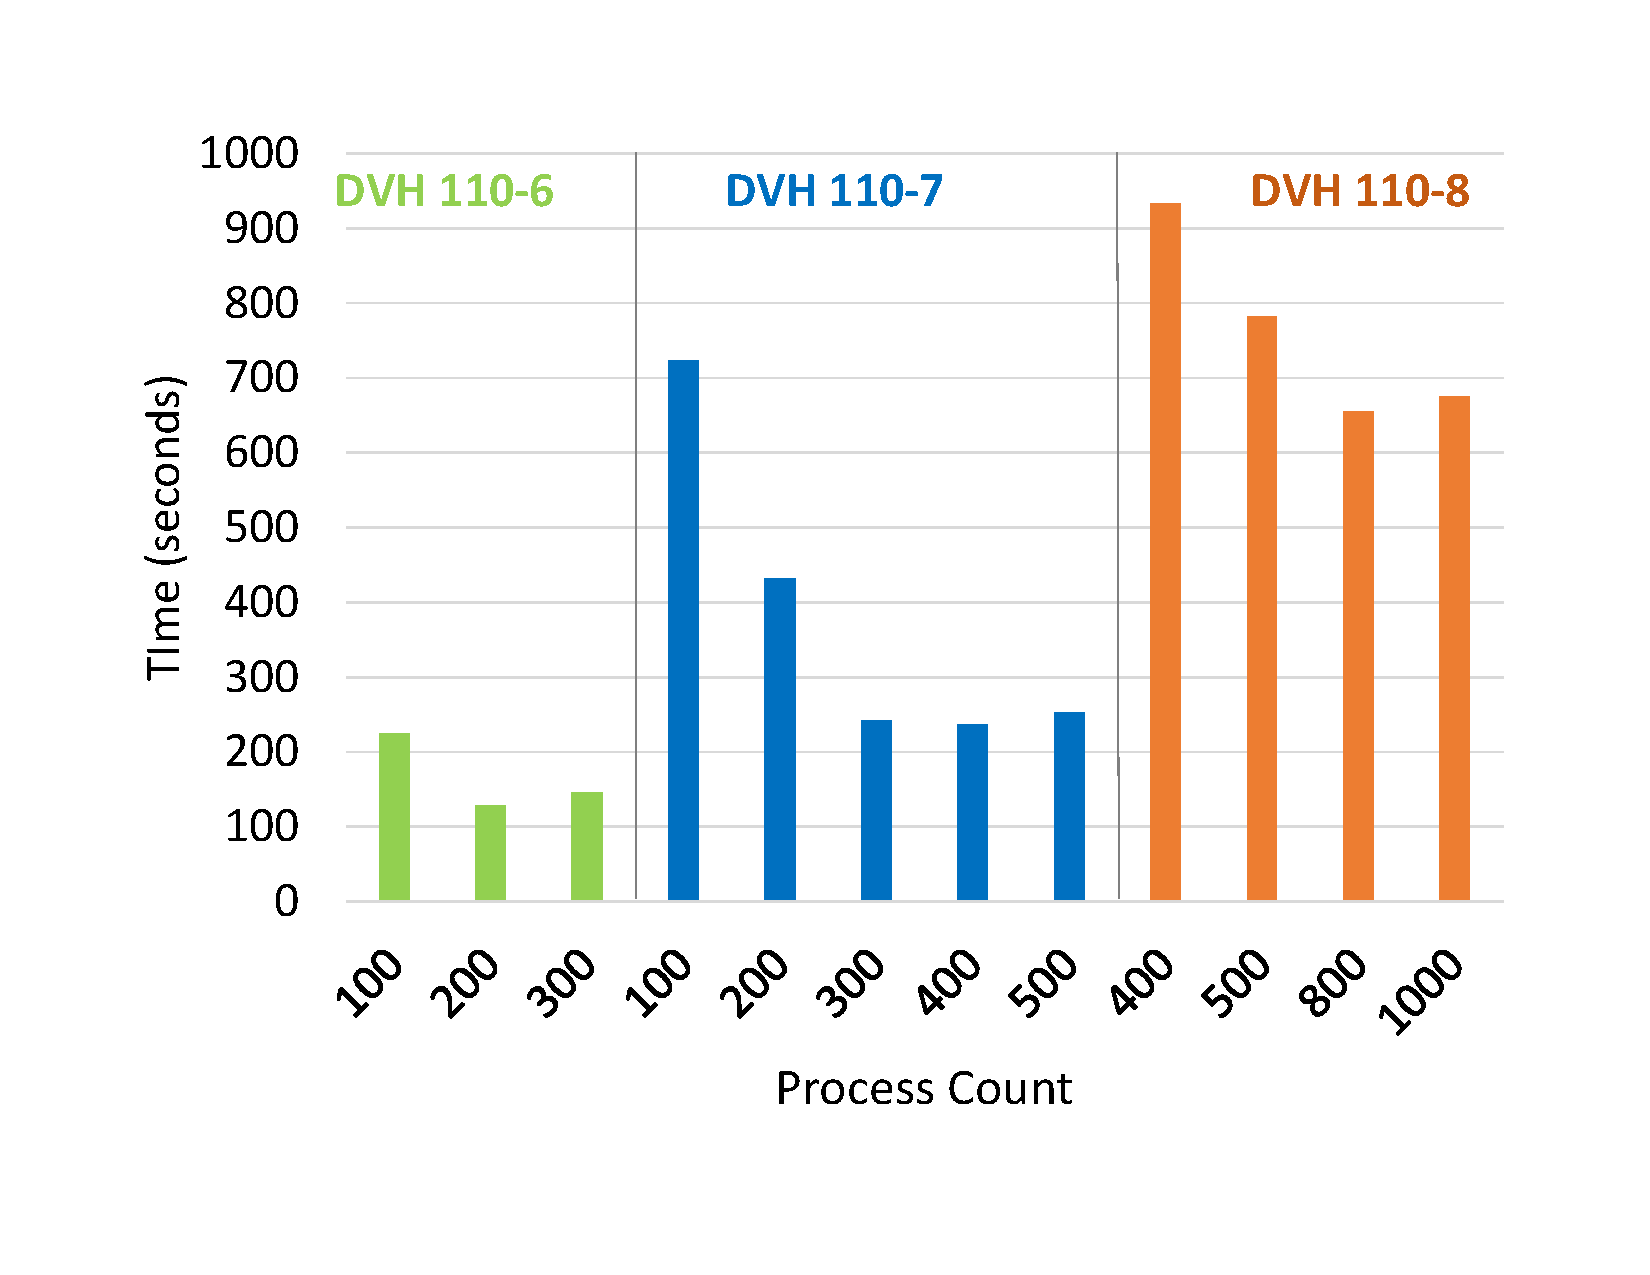
\includegraphics[width=0.5\textwidth, trim={2cm 2cm 2cm
    2cm},clip]{fig/dvh.pdf}
\end{center}
\vspace{-.15in}
\caption{Strong-scaling experiments on Theta.}
\label{fig:theta}
\vspace{-.2in}
\end{wrapfigure}

In recent years, several cloud providers have launched MPI-capabable
HPC nodes for their cloud services and significantly upgraded their
network
interconnects~\cite{azure-august2019,parallelcluster}. Alongside
related advances in cloud architectures and MPI implementations, this
move signals the ability for massively parallel analytics to be
deployed as a service in the near future. In this spirit, we also
conduct some preliminary strong-scaling experiments on the Theta
supercomputer. For this we used a fully monomorphized $m$-CFA
(distinct from the $m$-CFA used in the previous
subsection)---experiments we had ready to go when our allocation on
Theta became possible. The Theta Supercomputer~\cite{parker2017early}
at the Argonne Leadership Computing Facility (ALCF) of the Argonne
National Laboratory is a Cray machine with a peak performance of
$11.69$ petaflops. It is based on the second-generation Intel Xeon Phi
processor and is made up of 281,088 compute cores. It has an aggregate
of $843.264$ TiB of DDR4 RAM, $70.272$ TiB of MCDRAM and $10$ PiB of
online disk storage. The supercomputer has a Dragonfly network
topology uses the Lustre filesystem.


We ran three sets of $m$-CFA worst-case experiments with $110$ terms
and $m$ = $6$, $7$ and $8$. The results of the three sets of
experiments, referred to as \texttt{dvh-110-6}, \texttt{dvh-110-7} and
\texttt{dvh-110-8} are plotted in Figure~\ref{fig:theta}. For all
three set of experiments we observe improvement in performance with
increase in process counts, until maximum efficiency is attained,
after which performance degrades with increasing process counts, due
to communication overhead and workload starvation. In general, for a
given workload (problem size), we observe a range of processes that
exhibit healthy scalability. \texttt{dvh-110-6} shows a near $100\%$
scaling efficiency ($2\times$ speedup while increasing the process
count from $100$ to $200$), performance however drops when the number
of processes is increased to 300. Similarly, \texttt{dvh-110-7} shows
a $75\%$ scaling efficiency ($3\times$ speedup when the process count
is increased from $100$ to $400$), and \texttt{dvh-110-8} shows a
$71\%$ scaling efficiency ($1.42\times$ speedup going $400$ to $800$).

%Even though the largest problem is run at $2\times$ time process count,
%the scaling efficiency drops by only $4\%$, indicative of a robust and a
%scalable parallel deductive inference backend.\tom{last sentence is awful...}



